% !TEX TS-program = pdflatex
% !TEX encoding = UTF-8 Unicode

% This is a simple template for a LaTeX document using the "article" class.
% See "book", "report", "letter" for other types of document.

\documentclass[10pt,twocolumn]{article}

\usepackage[utf8]{inputenc} % set input encoding (not needed with XeLaTeX)
\usepackage{graphicx}
\usepackage{listings} 
\usepackage{xcolor,colortbl}
\usepackage[section]{placeins}
\usepackage{amsthm}
\usepackage{mathtools}
\graphicspath{ {images/} }

%%% Examples of Article customizations
% These packages are optional, depending whether you want the features they provide.
% See the LaTeX Companion or other references for full information.

%%% PAGE DIMENSIONS
\usepackage{geometry} % to change the page dimensions
\geometry{a4paper} % or letterpaper (US) or a5paper or....
\geometry{margin=0.55in} % for example, change the margins to 2 inches all round
% \geometry{landscape} % set up the page for landscape
%   read geometry.pdf for detailed page layout information

\usepackage{graphicx} % support the \includegraphics command and options

% \usepackage[parfill]{parskip} % Activate to begin paragraphs with an empty line rather than an indent

%%% PACKAGES
\usepackage{booktabs} % for much better looking tables
\usepackage{array} % for better arrays (eg matrices) in maths
\usepackage{paralist} % very flexible & customisable lists (eg. enumerate/itemize, etc.)
\usepackage{verbatim} % adds environment for commenting out blocks of text & for better verbatim
\usepackage{subfig} % make it possible to include more than one captioned figure/table in a single float
\usepackage{indentfirst}
\usepackage{amsfonts}
\usepackage{amssymb}
\usepackage{amsthm}
% These packages are all incorporated in the memoir class to one degree or another...

%%% HEADERS & FOOTERS
\usepackage{fancyhdr} % This should be set AFTER setting up the page geometry
\pagestyle{fancy} % options: empty , plain , fancy
\renewcommand{\headrulewidth}{0pt} % customise the layout...
\lhead{}\chead{}\rhead{}
\lfoot{}\cfoot{\thepage}\rfoot{}

%%% SECTION TITLE APPEARANCE
\usepackage{sectsty}
\allsectionsfont{\sffamily\mdseries\upshape} % (See the fntguide.pdf for font help)
% (This matches ConTeXt defaults)

%%% ToC (table of contents) APPEARANCE
\usepackage[nottoc,notlof,notlot]{tocbibind} % Put the bibliography in the ToC
\usepackage[titles,subfigure]{tocloft} % Alter the style of the Table of Contents
\renewcommand{\cftsecfont}{\rmfamily\mdseries\upshape}
\renewcommand{\cftsecpagefont}{\rmfamily\mdseries\upshape} % No bold!
\setlength{\parindent}{0.5cm} 

%%% END Article customizations

%%% The "real" document content comes below...

\title{On Middle Primes In Goldbach Partitions}
\author{Marcin Barylski}
\date{\small{Published: August 12, 2019 \\ The last update: September 3, 2019}}

\definecolor{Gray}{gray}{0.85}
\definecolor{LightCyan}{rgb}{0.88,1,1}
\newcolumntype{a}{>{\columncolor{Gray}}c}
\newcolumntype{b}{>{\columncolor{white}}c}

\newtheorem{theorem}{Theorem}
\newtheorem{lemma}[theorem]{Lemma}

\newcommand\bigforall{\mbox{\huge $\mathsurround0pt\forall$}} 
\newcommand\bigexists{\mbox{\huge $\mathsurround0pt\exists$}} 

\begin{document}
\maketitle

\begin{abstract}
Goldbach strong conjecture, still unsolved, states that all even integers $n \textgreater 2$ can be expressed as the sum of two prime numbers (Goldbach partitions of $n$). Let's call a pair of primes $(p_1, p_2)$ the middle primes of $n$ if and only if $p_1 + p_2 = n$ and $p_1$ is the greatest prime $\leq \frac{n}{2}$ and  $p_2$ is the smallest prime $\geq \frac{n}{2}$. This work is devoted to middle primes and their various properties.
\end{abstract}

\section{Introduction}

Goldbach strong conjecture ($GSC$, also called binary) asserts that all positive even integer $n$ $\geq$ 4 can be expressed as the sum of two prime numbers. This hypothesis, formulated by Goldbach in 1742 in letter to Euler \cite{goldbach1742} and then updated by Euler to the form above is one of the oldest and still unsolved problems in number theory. Empirical verification showed that it is true for all $n$ $\leq$ 4 x $10^{18}$ \cite{oliveira2012} \cite{oliveira2013}.\par
The expression of a given positive even number $n$ as a sum of two primes $p_1$ and $p_2$ is called a Goldbach Partition ($GP$) of $n$.  Let's denote this relation as $GSC(n, p_1, p_2)$. Then Goldbach strong conjecture can be written as (1):

\begin{equation}
\displaystyle\mathop{\bigforall}_{x \textgreater 1, x \in \mathbb{N}} \displaystyle\mathop{\bigexists}_{p_1, p_2 \in \mathbb{P}} GSC (2x, p_1, p_2)
\end{equation}

Let's call a pair of primes $(p_1, p_2)$ the middle primes of $n$ if and only if $p_1 + p_2 = n$ and $p_1$ is the greatest prime $\leq \frac{n}{2}$ and  $p_2$ is the smallest prime $\geq \frac{n}{2}$. Let's call $p_1$ the lesser middle prime (and denote it as $p_{ml}$) and $p_2$ - the greater middle prime ($p_{mg}$).

\section{Middle  primes in GSC}

If $n = 2p$ ($p \in \mathbb{P}$), then $p_{ml} = p_{mg} = p$. Based on Prime Number Theorem (which describes the asymptotic distribution of the prime numbers amongs other numbers) we have that if $n \to \infty$ then in a set $S_{all}$ of $n$ positive numbers we have $\approx \frac{n}{log (n)}$ primes.

\begin{lemma}
If even number has GP, then difference between middle primes is always even.
\end{lemma}
\begin{proof}
Let's assume that $n$ is even and $\textgreater 2$. According to GSC, such number has at least one GP. If $n=4$, then middle primes are $\{2, 2\}$, and difference between them is $0$. If $n \textgreater 4$, then all primes in GPs are odd, thus both middle primes ($p_{ml}$ and $p_{mg}$) are odd. Difference between two odd numbers is always even.
\end{proof}

\begin{figure}[!ht]
\centering
\captionsetup{justification=centering}
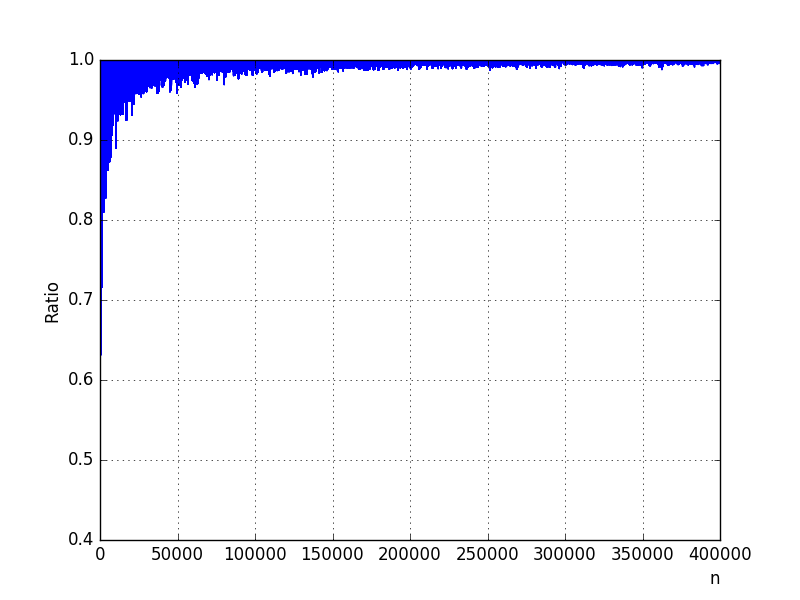
\includegraphics[width=9cm]{f_ratio_two_biggest_primes}
\caption[caption]{Ratio of $p_{ml}$ to $p_{mg}$ in $GP(n)$; $4 \leq n \leq 4 \times 10^5$}
\label{fig:middleprimesratio}
\end{figure}

\begin{figure}[!ht]
\centering
\captionsetup{justification=centering}
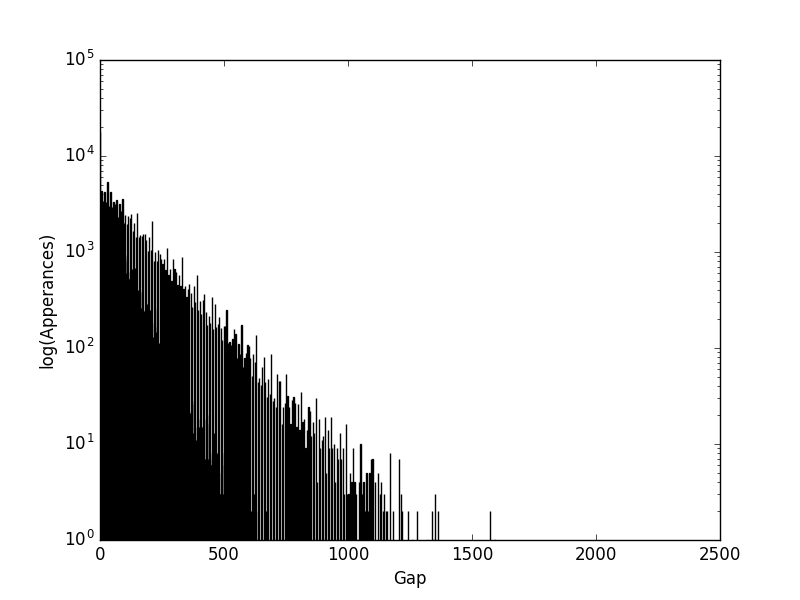
\includegraphics[width=9cm]{f_diff_in_middle_primes_freq}
\caption[caption]{Frequency of gap between $p_{mg}$ and $p_{ml}$ in $GP(n)$; $4 \leq n \leq 4 \times 10^5$}
\label{fig:middleprimesgapfreq}
\end{figure}

\section{Summary and next steps}

TBD

\begin{thebibliography}{9}
\bibitem{goldbach1742}
  Christian Goldbach, 
  \emph{On the margin of a letter to Leonard Euler},
  1742.
\bibitem{oliveira2012}
  Tomás Oliveira e Silva,
  \emph{Goldbach conjecture verification.}
  http://sweet.ua.pt/tos/goldbach.html,
  2012.
\bibitem{oliveira2013}
  Tomás Oliveira e Silva, Siegfried Herzog, and Silvio Pardi, 
  \emph{Empirical verification of the even Goldbach conjecture and computation of prime gaps up to 4 $\times 10^{18}$.}, 
  Mathematics of Computation, vol. 83, no. 288, pp. 2033-2060, 
  July 2014 (published electronically on November 18, 2013.
  
\end{thebibliography}

\end{document}
